\begin{figure}
\begin{center}
\begin{tabular}{l}
(a)
\begin{tikzpicture}
\begin{axis}[
  domain=0:3.14,
  axis lines = left,
  legend pos=outer north east,
  width=8cm,
  height=3cm,
  scale only axis,
]
\addplot [
  samples=100, 
  color=red,
]
{sin(deg(2*x))};

\end{axis}
\end{tikzpicture}

(b)
\begin{tikzpicture}
\begin{axis}[
  domain=0:6.28,
  axis lines = left,
  legend pos=outer north east,
  width=16cm,
  height=3cm,
  scale only axis,
]
\addplot [
  samples=100, 
  color=red,
]
{sin(deg(x))};

\end{axis}
\end{tikzpicture} \\

(c)
\begin{tikzpicture}
\begin{axis}[
  domain=0:3.14,
  axis lines = left,
  legend pos=outer north east,
  width=8cm,
  height=3cm,
  scale only axis,
]
\addplot [
  samples=100, 
  color=blue,
]
{sin(deg(2*x))};

\end{axis}
\end{tikzpicture}

(d)
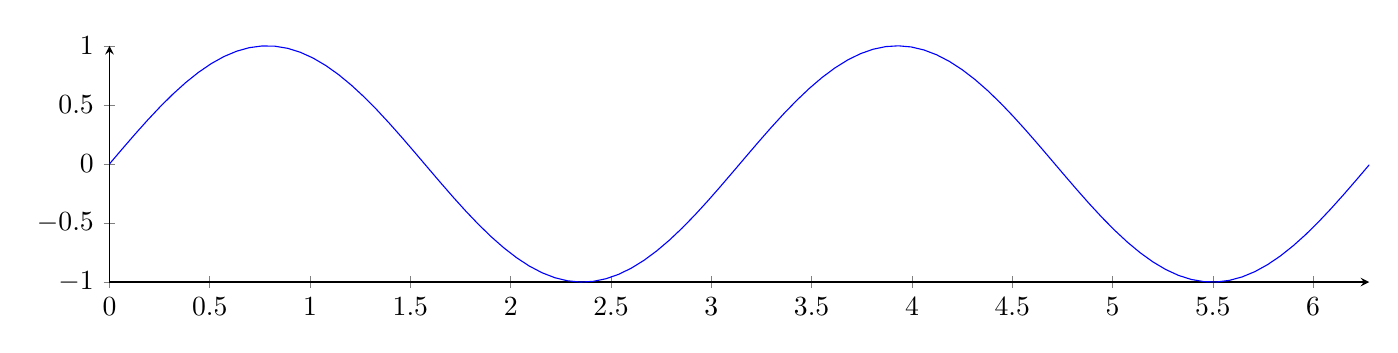
\begin{tikzpicture}
\begin{axis}[
  domain=0:6.28,
  axis lines = left,
  legend pos=outer north east,
  width=16cm,
  height=3cm,
  scale only axis,
]
\addplot [
  samples=100, 
  color=blue,
]
{sin(deg(2*x))};

\end{axis}
\end{tikzpicture}

\end{tabular}
\end{center}
\end{figure}
